\documentclass[../../main.tex]{subfiles}

\begin{document}

\chapter{Vectors and Geometry}

On my other notes on linear algebra, we discussed vectors and
vector spaces in detail. However, I wish to discuss some parts
again as linear algebra and multivariable calculus have different
perspectives on how we view them. In this note, let's discuss
more on the geometric interpretation and less on abstractness
of vector spaces.

\section{Basic Terms and Intuitions}

First, why should we even bother higher dimension for multivariable
calculus? As the name suggests, multivariable calculus studies
calculus over many variables. With generalization from the single
variable calculus concepts, it is natural to consider planes and
spaces of higher dimension. For instance, say we have a function
$f(x, y) = x + y$. We cannot graph this in the normal 2 dimensional
Cartesian plane as we have two inputs and an output while the plane
only has the space for two. As we have discussed in the notes for
linear algebra, we can graph such functions in a 3 dimensional
space.

The standard and conventional orientation of the 3D Cartesian
Coordinate System is \textbf{the Right-hand Rule}. The orientation
of the axis below follows the right-hand rule.

\begin{figure}[H]
\centering
\tdplotsetmaincoords{70}{110}
\begin{tikzpicture}[
        tdplot_main_coords,
        axis/.style={->,thick},
        scale=0.4
    ]
	\draw[axis] (-2,0,0) -- (8,0,0) node[left] {$x$};
	\draw[axis] (0,-1,0) -- (0,8,0) node[right] {$y$};
	\draw[axis] (0,0,-1) -- (0,0,8) node[left] {$z$};
\end{tikzpicture}
\end{figure}

One way to memorize this is to have your curled right hand face up.
Then, the direction where your hand is pointing is the direction of
the $x$-axis and the direction of your thumb is the direction of the
$z$-axis. This is a very common explanation; however, to be honest
it is quite hard to remember for me. Another explanation that really
helped me is to think of a clock at 3 P.M. The hour hand is the
$x$-axis and the minute hand is the $y$-axis. Then, if you draw
a line from the center of the clock pointing at you, that would
be the $z$-axis.

Besides having the name \textbf{3-dimensional Cartesian coordinate
system}, it is often called as \textbf{rectangular coordinate system
for 3-space}. When depicting a specific point, we will use the
ordered triple $(x, y, z)$.

Some fun facts that we can notice from the notation is that we can
represent $x$, $y$, and $z$ axis as $\{ (x, 0, 0) \mid x \in
\mathbb{R} \}$, $\{ (0, y, 0) \mid y \in \mathbb{R} \}$, and
$\{ (0, 0, z) \mid z \in \mathbb{R} \}$ respectively assuming that
we only consider real numbers.

An extension of the idea above are planes perpendicular to an axis.
We can see that the $xy$-plane, $yz$-plane, and $zx$-plane can be
represented as the following.

\begin{minipage}{0.3\textwidth}
\begin{center}
\textbf{$xy$-plane} \\
$\{ (x, y, 0) \mid x, y \in \mathbb{R} \}$
\end{center}
\begin{figure}[H]
\centering
\tdplotsetmaincoords{70}{110}
\begin{tikzpicture}[
        tdplot_main_coords,
        axis/.style={->,thick},
        scale=0.25
    ]
	\draw[axis] (-2,0,0) -- (8,0,0) node[left] {$x$};
	\draw[axis] (0,-1,0) -- (0,8,0) node[right] {$y$};
	\draw[axis] (0,0,-1) -- (0,0,8) node[left] {$z$};

    \fill[Blue, opacity=0.3]
        (-2,-1,0) -- (8,-1,0) -- (8,8,0) -- (-2,8,0) -- cycle;
\end{tikzpicture}
\end{figure}
\end{minipage}
\hfill
\begin{minipage}{0.3\textwidth}
\begin{center}
\textbf{$yz$-plane} \\
$\{ (0, y, z) \mid y, z \in \mathbb{R} \}$
\end{center}
\begin{figure}[H]
\centering
\tdplotsetmaincoords{70}{110}
\begin{tikzpicture}[
        tdplot_main_coords,
        axis/.style={->,thick},
        scale=0.25
    ]
	\draw[axis] (-2,0,0) -- (8,0,0) node[left] {$x$};
	\draw[axis] (0,-1,0) -- (0,8,0) node[right] {$y$};
	\draw[axis] (0,0,-1) -- (0,0,8) node[left] {$z$};

    \fill[Red, opacity=0.3]
        (0,-2,0) -- (0,8,0) -- (0,8,8) -- (0,-2,8) -- cycle;
\end{tikzpicture}
\end{figure}
\end{minipage}
\hfill
\begin{minipage}{0.3\textwidth}
\begin{center}
\textbf{$zx$-plane} \\
$\{ (x, 0, z) \mid x, z \in \mathbb{R} \}$
\end{center}
\begin{figure}[H]
\centering
\tdplotsetmaincoords{70}{110}
\begin{tikzpicture}[
        tdplot_main_coords,
        axis/.style={->,thick},
        scale=0.25
    ]
	\draw[axis] (-2,0,0) -- (8,0,0) node[left] {$x$};
	\draw[axis] (0,-1,0) -- (0,8,0) node[right] {$y$};
	\draw[axis] (0,0,-1) -- (0,0,8) node[left] {$z$};

    \fill[Yellow, opacity=0.3]
        (-2,0,0) -- (8,0,0) -- (8,0,8) -- (-2,0,8) -- cycle;
\end{tikzpicture}
\end{figure}
\end{minipage}

We can also notice that depending on what we have in the place
for $0$, we can have the planes $x = a$, $y = b$, and $z = c$.

One other extension that we can have from 2D plane is the distance
formula between two points.

\begin{theorem}{Distance Formula}{Distance Formula}
The distance between two points $(x_1, y_1, z_1)$ and
$(x_2, y_2, z_2)$ on a 3D plane can be represented as the following
equation.
\[
d
= \sqrt{ (x_2 - x_1)^2 + (y_2 - y_1)^2 + (z_2 - z_1)^2 }
\]
\end{theorem}
\begin{proof}
First, construct a right triangle with the points $A(x_1, y_1, z_1)$,
$B(x_2, y_2, \linebreak z_2)$, and $C(x_2, y_2, z_1)$. Notice that
the length of $BC = |z_2 - z_1|$ and the length of the segment $AC =
\sqrt{(x_2 - x_1)^2 + (y_2 - y_1)^2}$. Using the Pythagorean theorem,
\begin{align*}
    d
    &= \sqrt{
        \left( \sqrt{(x_2 - x_1)^2 + (y_2 - y_1)^2} \right)^2
            + (z_2 - z_1)^2
    } \\
    &= \sqrt{ (x_2 - x_1)^2 + (y_2 - y_1)^2 + (z_2 - z_1)^2 }
\end{align*}
holds and the distance between the two points can be written as
$\sqrt{ (x_2 - x_1)^2 + (y_2 - y_1)^2 + (z_2 - z_1)^2 }$.
\end{proof}

Using this, we can define a sphere just as we do for circles.

\subsection{Geometric Intuition in 3-Dimensions}

Consider equations of the following form with constants $G, H, I, J$.
\[
x^2 + y^2 + z^2 + Gx + Hy + Iz + J = 0
\]
Just as we use completing squares for circles, we can rewrite the
equation above as the following form with constants $a, b, c, K$.
\[
(x - a)^2 + (y - b)^2 + (z - c)^2 = K
\]
Square rooting both sides, we obtain
\[
\sqrt{(x - a)^2 + (y - b)^2 + (z - c)^2}
= \sqrt{K}
\]
which is equivalent of saying the locus of points $(x, y, z)$ that is
in the distance $\sqrt{K}$ from $(a, b, c)$ by Theorem
\ref{theo:Distance Formula}. Naturally, we can notice that if $K > 0$,
such sphere exists. If $K = 0$, the equation has one solution and
the graph is a single point. If $K < 0$, there exists no such graph.
Graphing a square with the center $(x_0, y_0, z_0)$ and radius $r$,
we can obtain the following by plotting the locus of $(x, y, z)$
that satisfy $(x - x_0)^2 + (y - y_0)^2 + (z - z_0)^2 = r^2$.

\begin{figure}[H]
\centering
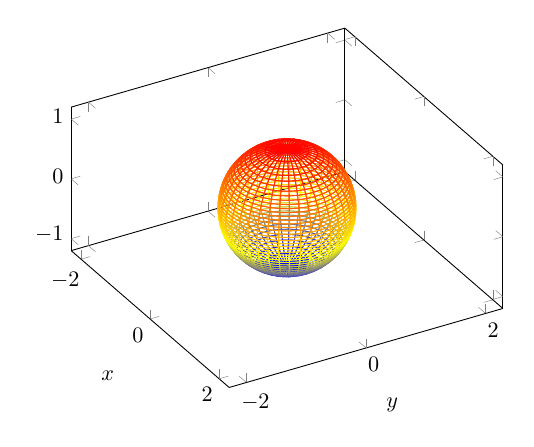
\begin{tikzpicture}[scale=0.8]
\begin{axis}[
    view={60}{30},
    axis equal,
    xlabel={$x$},ylabel={$y$}
]
\addplot3[
    mesh,z buffer=sort,
    samples=40,
    samples y=40,
    domain=-1:1,
    y domain=0:2*pi,
] (
    {sqrt(1-x^2) * cos(deg(y))},
    {sqrt(1-x^2) * sin(deg(y))},
    x
);
\end{axis}
\end{tikzpicture}
\end{figure}

Now that we can graph spheres, how about equations with two variables?
When you think about it, it is actually pretty simple since it is the
same as graphing in 2 dimensional plane and stretching it with respect
to the remaining axis. Such equations are known as
\textbf{cylindrical surface}.

\begin{figure}[H]
\centering
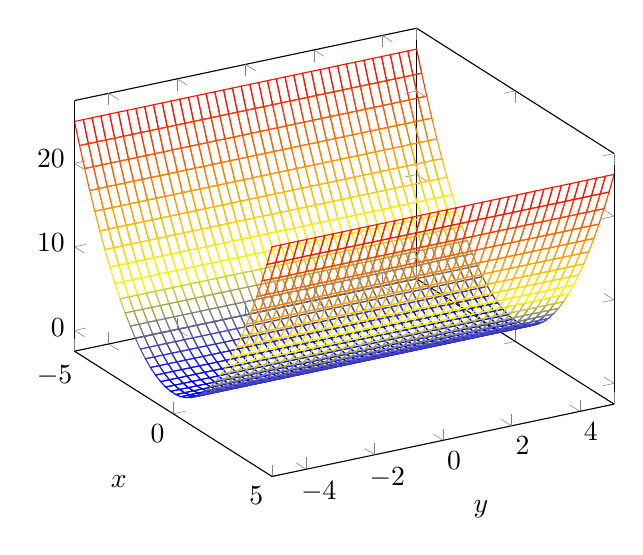
\begin{tikzpicture}
\begin{axis}[
    view={60}{30},
    xlabel={$x$},ylabel={$y$}
]
\addplot3[mesh,samples=40] {x^2};
\end{axis}
\end{tikzpicture}
\end{figure}

The graph above is $z = x^2$. This is the same as graphing the
quadratic function in $xz$-plane and making its copy across the
$y$-axis.

Continuing with this intuition, we can implement the ideas with
vectors.

\end{document}


